\section{Alle Stände}

\subsection{Finanzierung}

\begin{frame}[c]{Auslagen}
    \begin{itemize}[<+(1)->]
        \item Zelte etc. werden von uns gemietet
        \item Alle Getränkematerialien werden auf Kommission gekauft
        \item Dafür zahlt ihr nichts
        \item Hoffnung auf ausreichend Gewinn durch Verkauf
        \item Übriggebliebene Getränke werden zurückggeben
        \item Offene Getränke werden bei Helferparty verwendet
    \end{itemize}
\end{frame}

\begin{frame}[c]{Gewinnbeteiligung}
    Entlohnung proportional zu ...
    \begin{itemize}[<+(1)->]
        \item Unifest Gesamtgewinn
        \item Geleisteten Helferstunden
        \item (negativ) überproportionalem Schankverlust ;)
    \end{itemize}
\end{frame}


\subsection{Standbetreuer}

\begin{frame}[c]{Standbetreuer}
    \begin{itemize}[<+(1)->]
        \item Jeder Stand hat zwei Standbetreuer
        \item Es wird noch eine separate Einführung für Standbetreuer geben
        \item Koordinieren Auf-, Abbau und Betrieb
        \item Es ist \textbf{zu jedem Zeitpunkt} ein Betreuer am Stand
        \item Standbetreuer bleiben während des gesamten Festbetriebs \textbf{nüchtern}!
    \end{itemize}
\end{frame}



\subsection{Verteilung}

\begin{frame}[c]{Ständeverteilung}
    \begin{itemize}[<+(1)->]
        \item Ihr gebt eure Präferenz an 
            \begin{itemize}[<+(1)->]
                \item Typ (Bierausschank, Longdrinkstand oder eigener Stand)
                \item Ort (Forum, Otto-Amann-Platz oder Paulcke-Platz)
            \end{itemize}
        \item Bei eigenem Stand: Was ihr für Getränke anbieten wollt
        \item Wir verteilen eigene Stände thematisch sinnvoll
        \item Kleinere Gruppen sollten sich mit anderen zusammentun
        \item Weitere Wünsche können gerne geäußert werden
    \end{itemize}
\end{frame}



\subsection{Infrastruktur}

\begin{frame}[c]{Pavillion}
    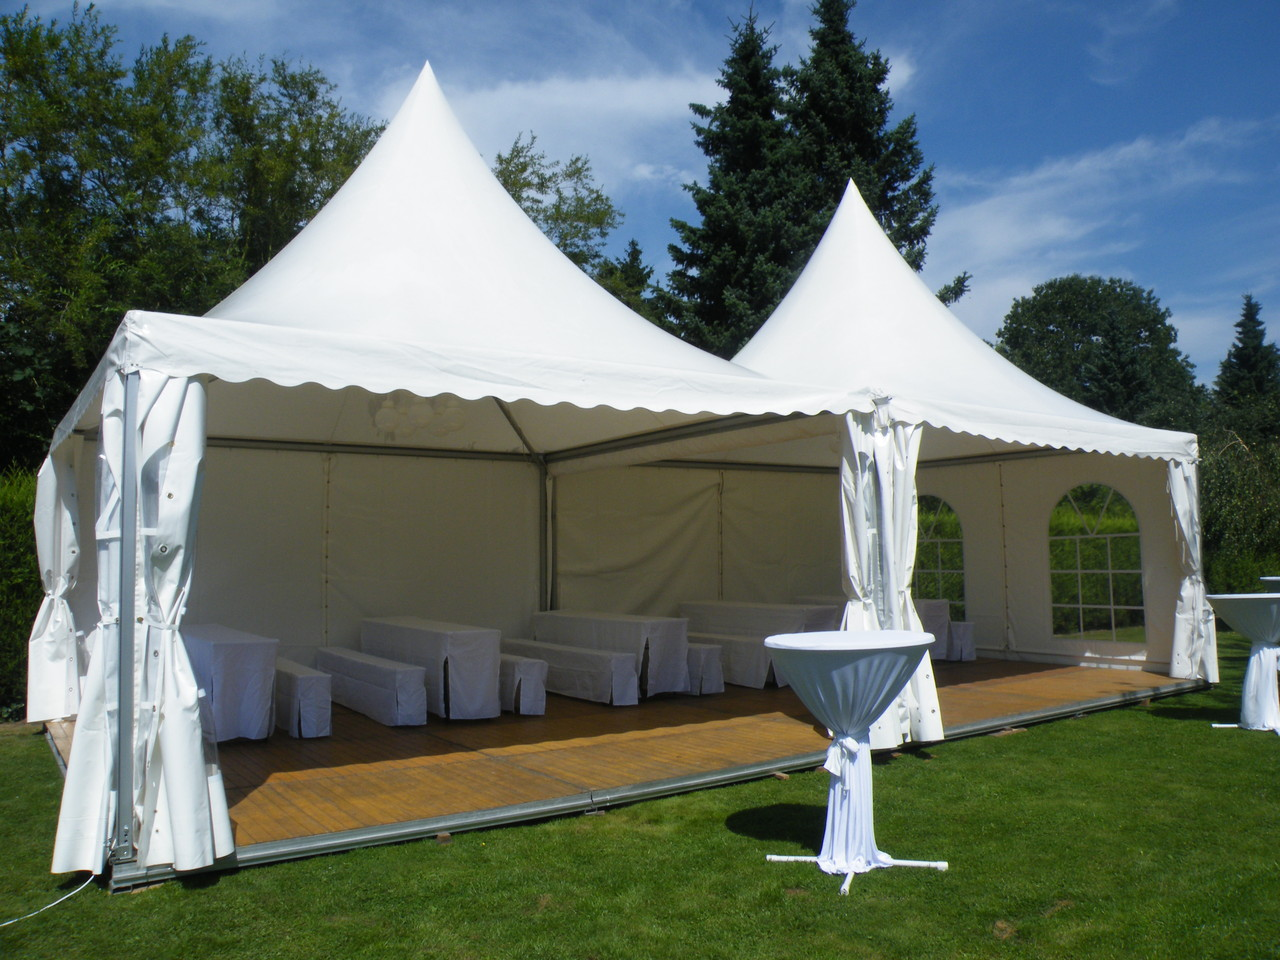
\includegraphics[width=\textwidth]{Zelte}
\end{frame}


\begin{frame}[c]{Standardtresen}
    % trim = l b r t
    \includegraphics[width=\textwidth,clip,trim = 350 50 150 200]{tresen}
\end{frame}


\begin{frame}[c]{Infrastruktur}
    \begin{itemize}
        \item Pavillion
        \item Standardtresen aus Biertischgarnituren
        \item Kasse mit Wechselgeld
        \item Stromanschluss (in sinnvollem Rahmen)
        \item 2 Biertische als Zubereitungsfläche
        \item 2 Bierbänke als Sitzgelegenheit
        \item Hygienepaket (Handwaschkanister, Handschuhe, Waschlappen, Eimer, Desinfektion, Seife etc.)
        \item Rolle Müllbeutel
        \item 1-2 Baustrahler % (Es wird versucht: LED-Ketten)
    \end{itemize}
\end{frame}



\subsection{Standbesetzung}

{
    \setbeamercolor{background canvas}{bg=}
    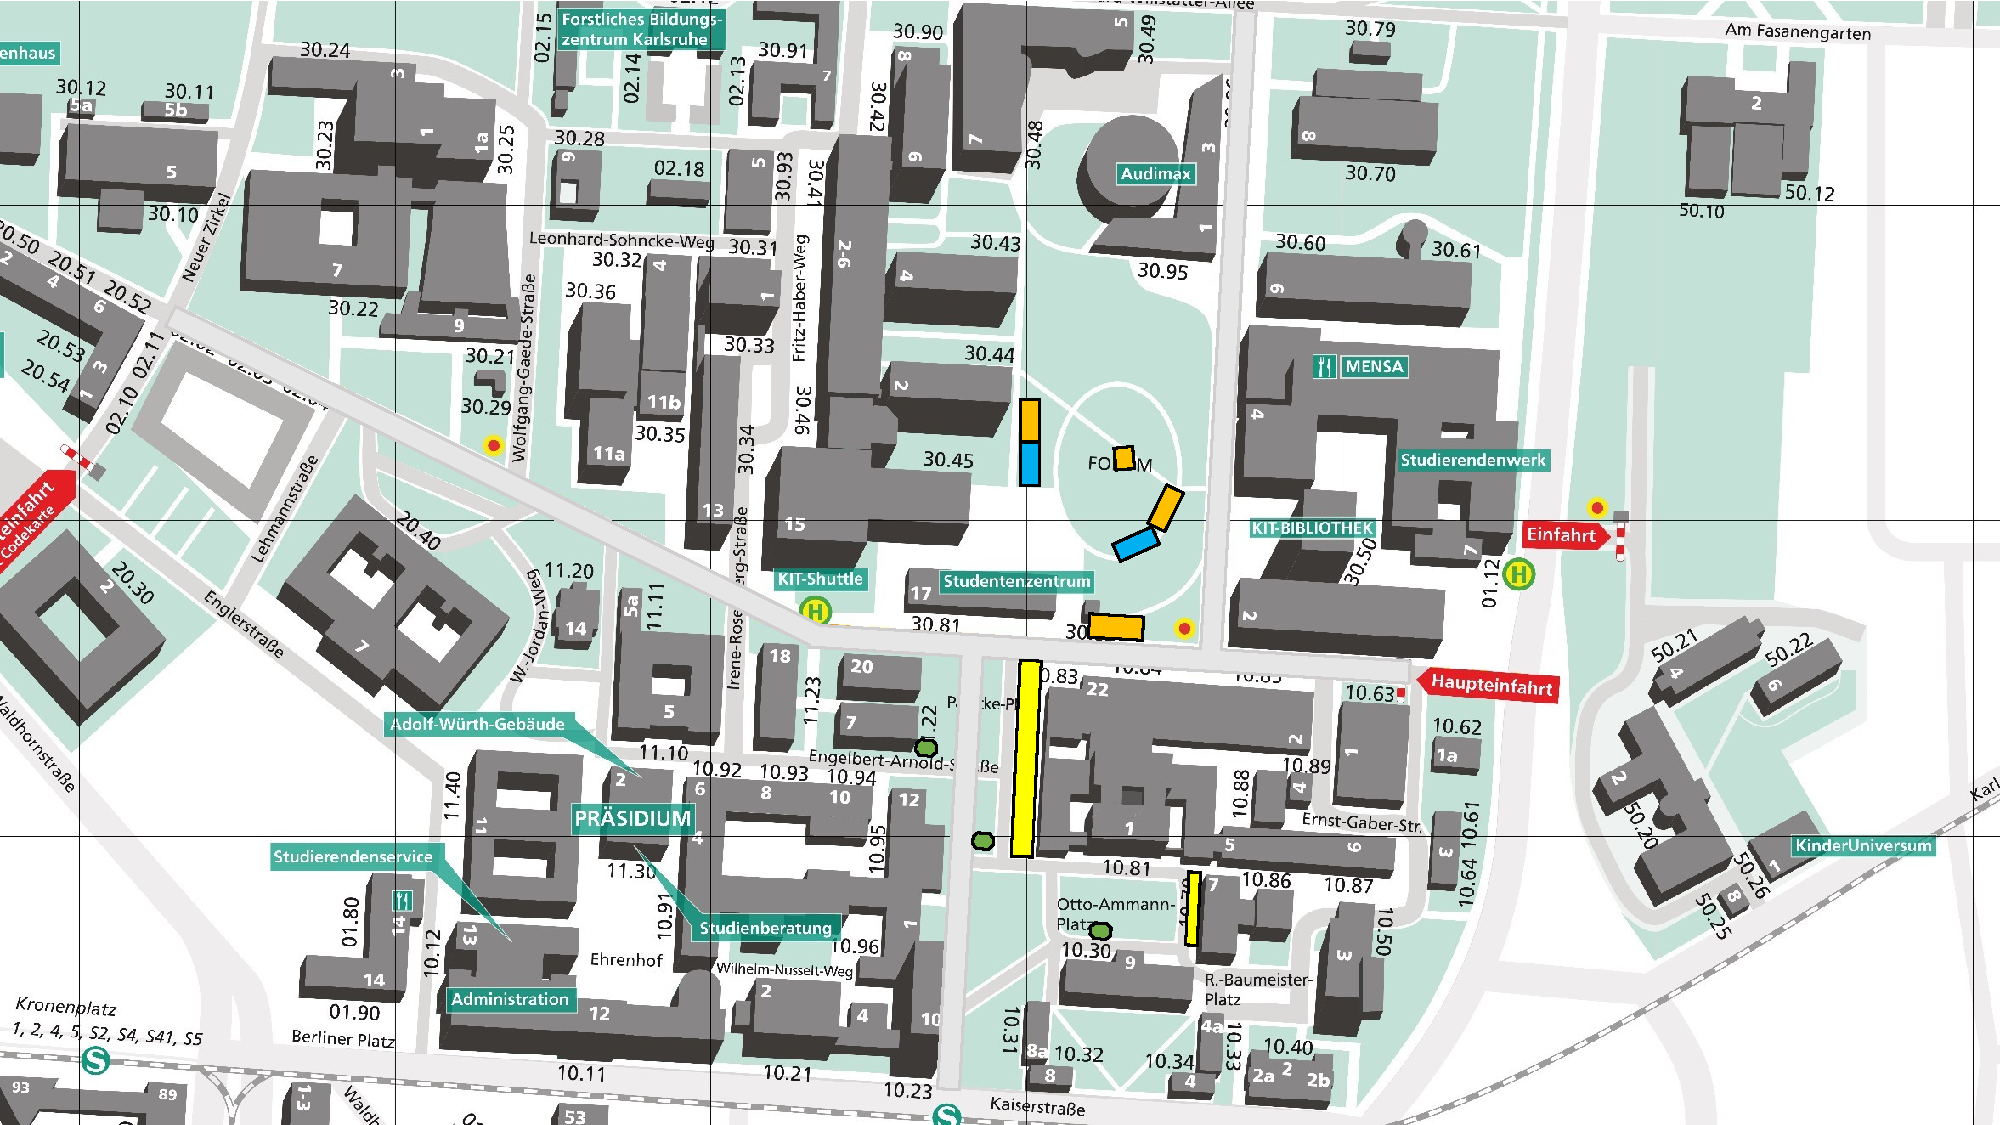
\includepdf[pages=-,frame]{BiMi_Treffen_Folien_3_7.pdf}
}

\begin{frame}[c]{Standbesetzung}
    \small
    \begin{tabular}{l|ll|ll}
        \textbf{Was und Wo?}& \multicolumn{2}{c}{\textbf{Nachmittag}} & \multicolumn{2}{c}{\textbf{Abends}} \\
        & Mixend    & Verkauf & Mixend    & Verkauf \\
        \hline
        Forum FOH         & 4 & 4 & 6 & 8 \\
        Forum Longdrink   & 3 & 3 & 8 & 6 \\
        Forum Bier        & 4 & 4 & 6 & 6 \pause \\
        \hline
        AKK-Bierinsel       & 8 & 8 & 8 & 8 \\
        Bierinsel           & 4 & 4 & 4 & 4 \\
        Eigener Stand 3x3   & 2 & 1 & 3 & 2 \\
        Eigener Stand 4x4   & 2 & 2 & 4 & 4 \\

    \end{tabular}
\end{frame}



\subsection{Eigene Stände}

% \subsubsection{Standangebote}

\begin{frame}[c]{Standangebote eigene Stände}
    \begin{itemize}[<+(1)->]
        \item Für 0.4L Becher oder Shotgläser
        \item Idealerweise etwas zu Trinken
        \item Kein Bier (es gibt genug Bierinseln)
        \item Keine Longdrinks (!)
        \item Muss nicht alkfrei sein (Bieten Bierinseln an)
        \item Idealerweise: Ein fancy Cocktail (gerne in Variation)
        \item Oder: Mehrere Shots
        \item Oder: Craftbeer, Met, Wein-Whisky, ...
    \end{itemize}
\end{frame}



\begin{frame}[c]{Standangebote eigene Stände}
    Feste Regeln für alle Stände:
    \begin{itemize}[<+(1)->]
        \item Allergenübersicht muss zur direkten Einsicht verfügbar sein!
        \item Bei Cocktails:
            \begin{itemize}[<+(1)->]
                \item Keine Sahne!
                \item Keine Milch!
                \item Keine Eier!
            \end{itemize}
    \end{itemize}
\end{frame}



\begin{frame}[c]{Mehr als normales Licht?}
    \begin{itemize}[<+(1)->]
        \item Es gibt jemanden der sich genau darum kümmert!
        \item Fragt Tom!
        \item (\mailto{tom.wolf@asta-kit.de})
    \end{itemize}
\end{frame}


\begin{frame}[c]{Was mit Holz?}
    \begin{itemize}[<+(1)->]
        \item Ihr wollt mehr haben als einen Standardstand, und es soll irgendwie aus Holz sein?
        \item Es gibt da Leute die euch mit der Planung Helfen können!
        \item Fragt Valle!
        \item (\mailto{valentin.haas@asta-kit.de})
    \end{itemize}
\end{frame}






